\documentclass[11pt]{article}
\def\figlang{fr}
\usepackage[a4paper,top=2.4cm,bottom=2.4cm,left=2.3cm,right=2.3cm,headsep=0.8cm,footskip=1cm]{geometry}
% Compatible XeLaTeX / LuaLaTeX (recommandé) et pdfLaTeX
\usepackage{iftex}
\ifPDFTeX
  \usepackage[T1]{fontenc}
  \usepackage[utf8]{inputenc}
  \usepackage{textcomp}
  \IfFileExists{tgtermes.sty}{\usepackage{tgtermes}}{\usepackage{mathptmx}}
  \IfFileExists{tgheros.sty}{\usepackage{tgheros}}{\usepackage[scaled=0.92]{helvet}}
\else
  \usepackage{fontspec}
  \setmainfont{TeX Gyre Termes}
  \setsansfont{TeX Gyre Heros}
\fi
\usepackage{amsmath,amssymb}
\usepackage{graphicx,booktabs,tabularx,array,multirow,float,enumitem}
\usepackage[table]{xcolor}
% Version de soumission : texte en noir sur fond blanc
\definecolor{navy}{HTML}{000000}\definecolor{ora}{HTML}{000000}\definecolor{fond}{HTML}{FFFFFF}
\usepackage[font=small,labelfont={bf,sf,color=navy},labelsep=period,justification=justified,singlelinecheck=false]{caption}
\captionsetup[table]{position=top,skip=4pt}
\usepackage{titlesec}
\titleformat{\section}{\sffamily\large\bfseries\color{navy}}{\thesection.}{0.5em}{}
\titleformat{\subsection}{\sffamily\normalsize\bfseries\color{navy}}{\thesubsection.}{0.5em}{}
\titleformat{\subsubsection}{\sffamily\normalsize\itshape\color{navy}}{\thesubsubsection.}{0.5em}{}
\titlespacing*{\section}{0pt}{14pt}{6pt}\titlespacing*{\subsection}{0pt}{10pt}{4pt}\titlespacing*{\subsubsection}{0pt}{8pt}{3pt}
\usepackage{fancyhdr}\pagestyle{fancy}\fancyhf{}
\renewcommand{\headrulewidth}{0.4pt}
\usepackage{tcolorbox}
\usepackage[hidelinks]{hyperref}
\usepackage{microtype}
\setlength{\parskip}{2pt}\setlength{\emergencystretch}{2em}\setlength{\parindent}{1.2em}
\linespread{1.06}
\setlist{itemsep=1pt,topsep=3pt,leftmargin=1.6em}
\renewcommand{\arraystretch}{1.15}
\newcommand{\fig}[3]{\begin{figure}[!htbp]\centering\includegraphics[width=#2\linewidth]{figures/\figlang_#1.png}\caption{#3}\label{fig:#1}\end{figure}}
\newcolumntype{R}{>{\raggedleft\arraybackslash}X}
\newcolumntype{L}{>{\raggedright\arraybackslash}X}

\ifPDFTeX\usepackage[french]{babel}\else\usepackage{polyglossia}\setmainlanguage{french}\fi
\usepackage{rotating}
\hypersetup{colorlinks=true,linkcolor=black,urlcolor=black,citecolor=black}
\fancyhead[L]{\sffamily\footnotesize\color{navy} Pluie et fièvre typhoïde au Sahel camerounais}
\fancyhead[R]{\sffamily\footnotesize\color{navy} Kazoune Bouba et al.}
\fancyfoot[C]{\sffamily\footnotesize\thepage}
\begin{document}\sloppy
\thispagestyle{fancy}
\noindent{\sffamily\footnotesize\color{ora}\textbf{ARTICLE DE RECHERCHE}\hfill\color{navy} Accès ouvert}\par\vspace{2pt}
\noindent{\color{navy}\rule{\linewidth}{1.2pt}}\par\vspace{8pt}
{\raggedright\sffamily\bfseries\LARGE\color{navy}Influence de la pluviométrie sur la dynamique et la prévision de la fièvre typhoïde au Sahel camerounais\par}
\vspace{4pt}
{\raggedright\sffamily\large\color{navy}De la modélisation mathématique à l'apprentissage automatique, à partir des données de surveillance de l'Extrême-Nord (2019-2025)\par}
\vspace{10pt}
\noindent{\sffamily\normalsize Kazoune Bouba Israel\textsuperscript{1,2,*}, Maïrousgou Céline\textsuperscript{1}, Kolaye Guilsou Gabriel\textsuperscript{2}\par}
\vspace{4pt}
\noindent{\footnotesize\textsuperscript{1}\,Délégation régionale de la santé publique de l'Extrême-Nord, Maroua, Cameroun\\
\textsuperscript{2}\,École nationale supérieure polytechnique de Maroua, Université de Maroua, Maroua, Cameroun\\
\textsuperscript{*}\,Auteur correspondant : [adresse électronique]\par}
\vspace{10pt}
\begin{tcolorbox}[colback=white,colframe=black,boxrule=0.5pt,arc=0pt,left=8pt,right=8pt,top=6pt,bottom=6pt,fontupper=\small]
{\sffamily\bfseries\color{navy}Résumé}\par\vspace{3pt}
\textbf{Contexte.} La fièvre typhoïde est l'une des maladies les plus déclarées dans l'Extrême-Nord du Cameroun, région sahélienne à saison des pluies unique. Nous avons étudié l'influence de la pluie sur sa dynamique et évalué si la pluie aide à prévoir les cas, afin d'orienter la préparation des districts de santé.\par
\textbf{Méthodes.} Nous avons analysé 417\,910 cas déclarés dans le DHIS2 par 522 formations sanitaires de 32 districts (2019-2025), combinés aux précipitations satellitaires. Un modèle de transmission à réservoir environnemental, dans lequel la pluie contamine l'eau, a servi à formuler les hypothèses. Le lien entre pluie et cas a été mesuré après retrait de la tendance, en distinguant le calendrier de la saison de son intensité. Plusieurs méthodes de prévision, avec et sans pluie, ont été évaluées sur trois années (2023-2025) et comparées par le test de Diebold-Mariano.\par
\textbf{Résultats.} Le pic des cas survenait en octobre, environ deux mois après le pic des pluies d'août (corrélation maximale de 0,54 à 8 semaines). En revanche, une saison plus pluvieuse que la normale n'entraînait pas davantage de cas, et l'ajout de la pluie n'améliorait pas la prévision. Un modèle d'apprentissage commun aux 32 districts réduisait l'erreur de prévision de 15\,\% à 4 semaines par rapport à la méthode de référence ($p<0{,}001$). La hausse des cas entre 2019 et 2022 coïncidait avec un triplement du nombre de formations déclarantes.\par
\textbf{Conclusion.} La pluie fixe le calendrier de la saison de typhoïde, mais non son intensité : la préparation des districts peut être planifiée dès juillet, tandis que la réduction des pics passe par l'eau, l'assainissement et le diagnostic.\par\vspace{3pt}
\textbf{Mots-clés :} fièvre typhoïde ; pluviométrie ; saisonnalité ; modélisation mathématique ; prévision ; surveillance ; DHIS2 ; Sahel ; Cameroun
\end{tcolorbox}

\begin{tcolorbox}[colback=white,colframe=black,boxrule=0.5pt,arc=0pt,left=8pt,right=8pt,top=5pt,bottom=5pt,fontupper=\small]
{\sffamily\bfseries\color{ora}Messages clés}\par\vspace{2pt}
\textbf{Ce que l'on savait.} La typhoïde se transmet par l'eau contaminée et augmente pendant la saison des pluies dans plusieurs pays ; les données africaines restent rares.\par
\textbf{Ce que cette étude apporte.} Dans l'Extrême-Nord du Cameroun, le pic de typhoïde survient environ deux mois après celui des pluies, de façon régulière sur sept ans ; la pluie annonce \textit{quand} la saison arrive, pas \textit{combien} de cas il y aura. Un modèle unique pour les 32 districts prévoit les cas à un mois mieux que les méthodes classiques.\par
\textbf{Implications pour la pratique.} Préparer les districts dès juillet ; cibler en priorité les districts où le lien avec la pluie est le plus net ; renforcer la déclaration dans les districts à données incomplètes ; ne pas interpréter la hausse des cas du DHIS2 sans tenir compte de l'extension du réseau.
\end{tcolorbox}

\section{Introduction}
La fièvre typhoïde, due à \textit{Salmonella enterica} sérovar Typhi, se transmet par l'eau et les aliments contaminés par des matières fécales. Elle cause chaque année plusieurs millions de cas et plus de 100\,000 décès, principalement en Asie du Sud et en Afrique subsaharienne [\hyperlink{ref1}{1},\hyperlink{ref2}{2}]. En Afrique subsaharienne, son fardeau reste mal mesuré, car le diagnostic repose souvent sur la clinique ou sur le test de Widal, peu spécifique [\hyperlink{ref3}{3}].

Dans l'Extrême-Nord du Cameroun, zone sahélienne à saison des pluies unique, la typhoïde figure parmi les maladies les plus déclarées dans le système de surveillance hebdomadaire DHIS2 [\hyperlink{ref4}{4}]. La pluie y joue un rôle a priori central : elle provoque le ruissellement, le débordement des latrines et la contamination des puits et des mares, principales sources d'eau de nombreux ménages. Comprendre comment la pluie influence la typhoïde, et si elle permet d'en anticiper les cas, aiderait directement les équipes de district à planifier leur réponse.

Deux approches complémentaires permettent d'étudier cette influence. Les modèles mathématiques de transmission décrivent les mécanismes, notamment l'accumulation des bactéries dans l'environnement [\hyperlink{ref5}{5},\hyperlink{ref6}{6}], mais leurs paramètres sont rarement connus localement. Les méthodes statistiques et d'apprentissage automatique apprennent directement des données observées et ont été utilisées pour prévoir la typhoïde en Inde, dans plusieurs pays à revenu élevé et au Népal, où elle a été associée aux précipitations et aux inondations [\hyperlink{ref7}{7}--\hyperlink{ref9}{9}]. Ces travaux concernent toutefois rarement l'Afrique, et leurs comparaisons de méthodes reposent souvent sur une seule période test, sans référence simple ni test statistique [\hyperlink{ref10}{10}].

Cette étude relie ces deux approches. À partir d'un modèle de transmission dans lequel la pluie contamine l'eau, nous testons trois questions : (i) la saison de typhoïde suit-elle la saison des pluies, et avec quel décalage ? (ii) une saison plus pluvieuse que la normale entraîne-t-elle davantage de cas ? (iii) la pluie améliore-t-elle la prévision des cas, et quelle méthode de prévision convient le mieux à l'échelle des districts ?

\section{Matériels et méthodes}
\subsection{Zone d'étude}
L'étude a été menée dans la région de l'Extrême-Nord du Cameroun, la plus septentrionale du pays, située entre 10° et 13° de latitude nord et entre 13° et 16° de longitude est (figure~\ref{fig:f2a_reference}). D'une superficie d'environ 34\,263 km², elle est frontalière du Nigeria à l'ouest et du Tchad à l'est, et touche le lac Tchad au nord. Elle était organisée en 32 districts de santé sur la période étudiée, répartis entre ses six départements : Diamaré (Bogo, Gazawa, Maroua 1, Maroua 2, Maroua 3, Méri, Petté), Logone-et-Chari (Fotokol, Goulfey, Kousséri, Mada, Makary), Mayo-Danay (Guéré, Kar-Hay, Maga, Vélé, Yagoua), Mayo-Kani (Guidiguis, Kaélé, Mindif, Moulvoudaye, Moutourwa), Mayo-Sava (Kolofata, Mora, Tokombéré) et Mayo-Tsanaga (Bourha, Hina, Koza, Mogodé, Mokolo, Mozogo, Roua).

La région connaît un climat sahélo-soudanien, avec une longue saison sèche d'octobre à mai et une saison des pluies courte mais intense de juin à septembre. Une grande partie de la population s'approvisionne en eau dans des puits, des forages et des mares, exposés au ruissellement pendant la saison des pluies. La région est en outre touchée par l'insécurité liée aux groupes armés et par des déplacements de population, qui fragilisent l'accès aux soins et la régularité des déclarations dans certains districts frontaliers. Ces caractéristiques font de l'Extrême-Nord un terrain particulièrement pertinent pour étudier le lien entre pluie et maladies hydriques.

\begin{sidewaysfigure}[p]\centering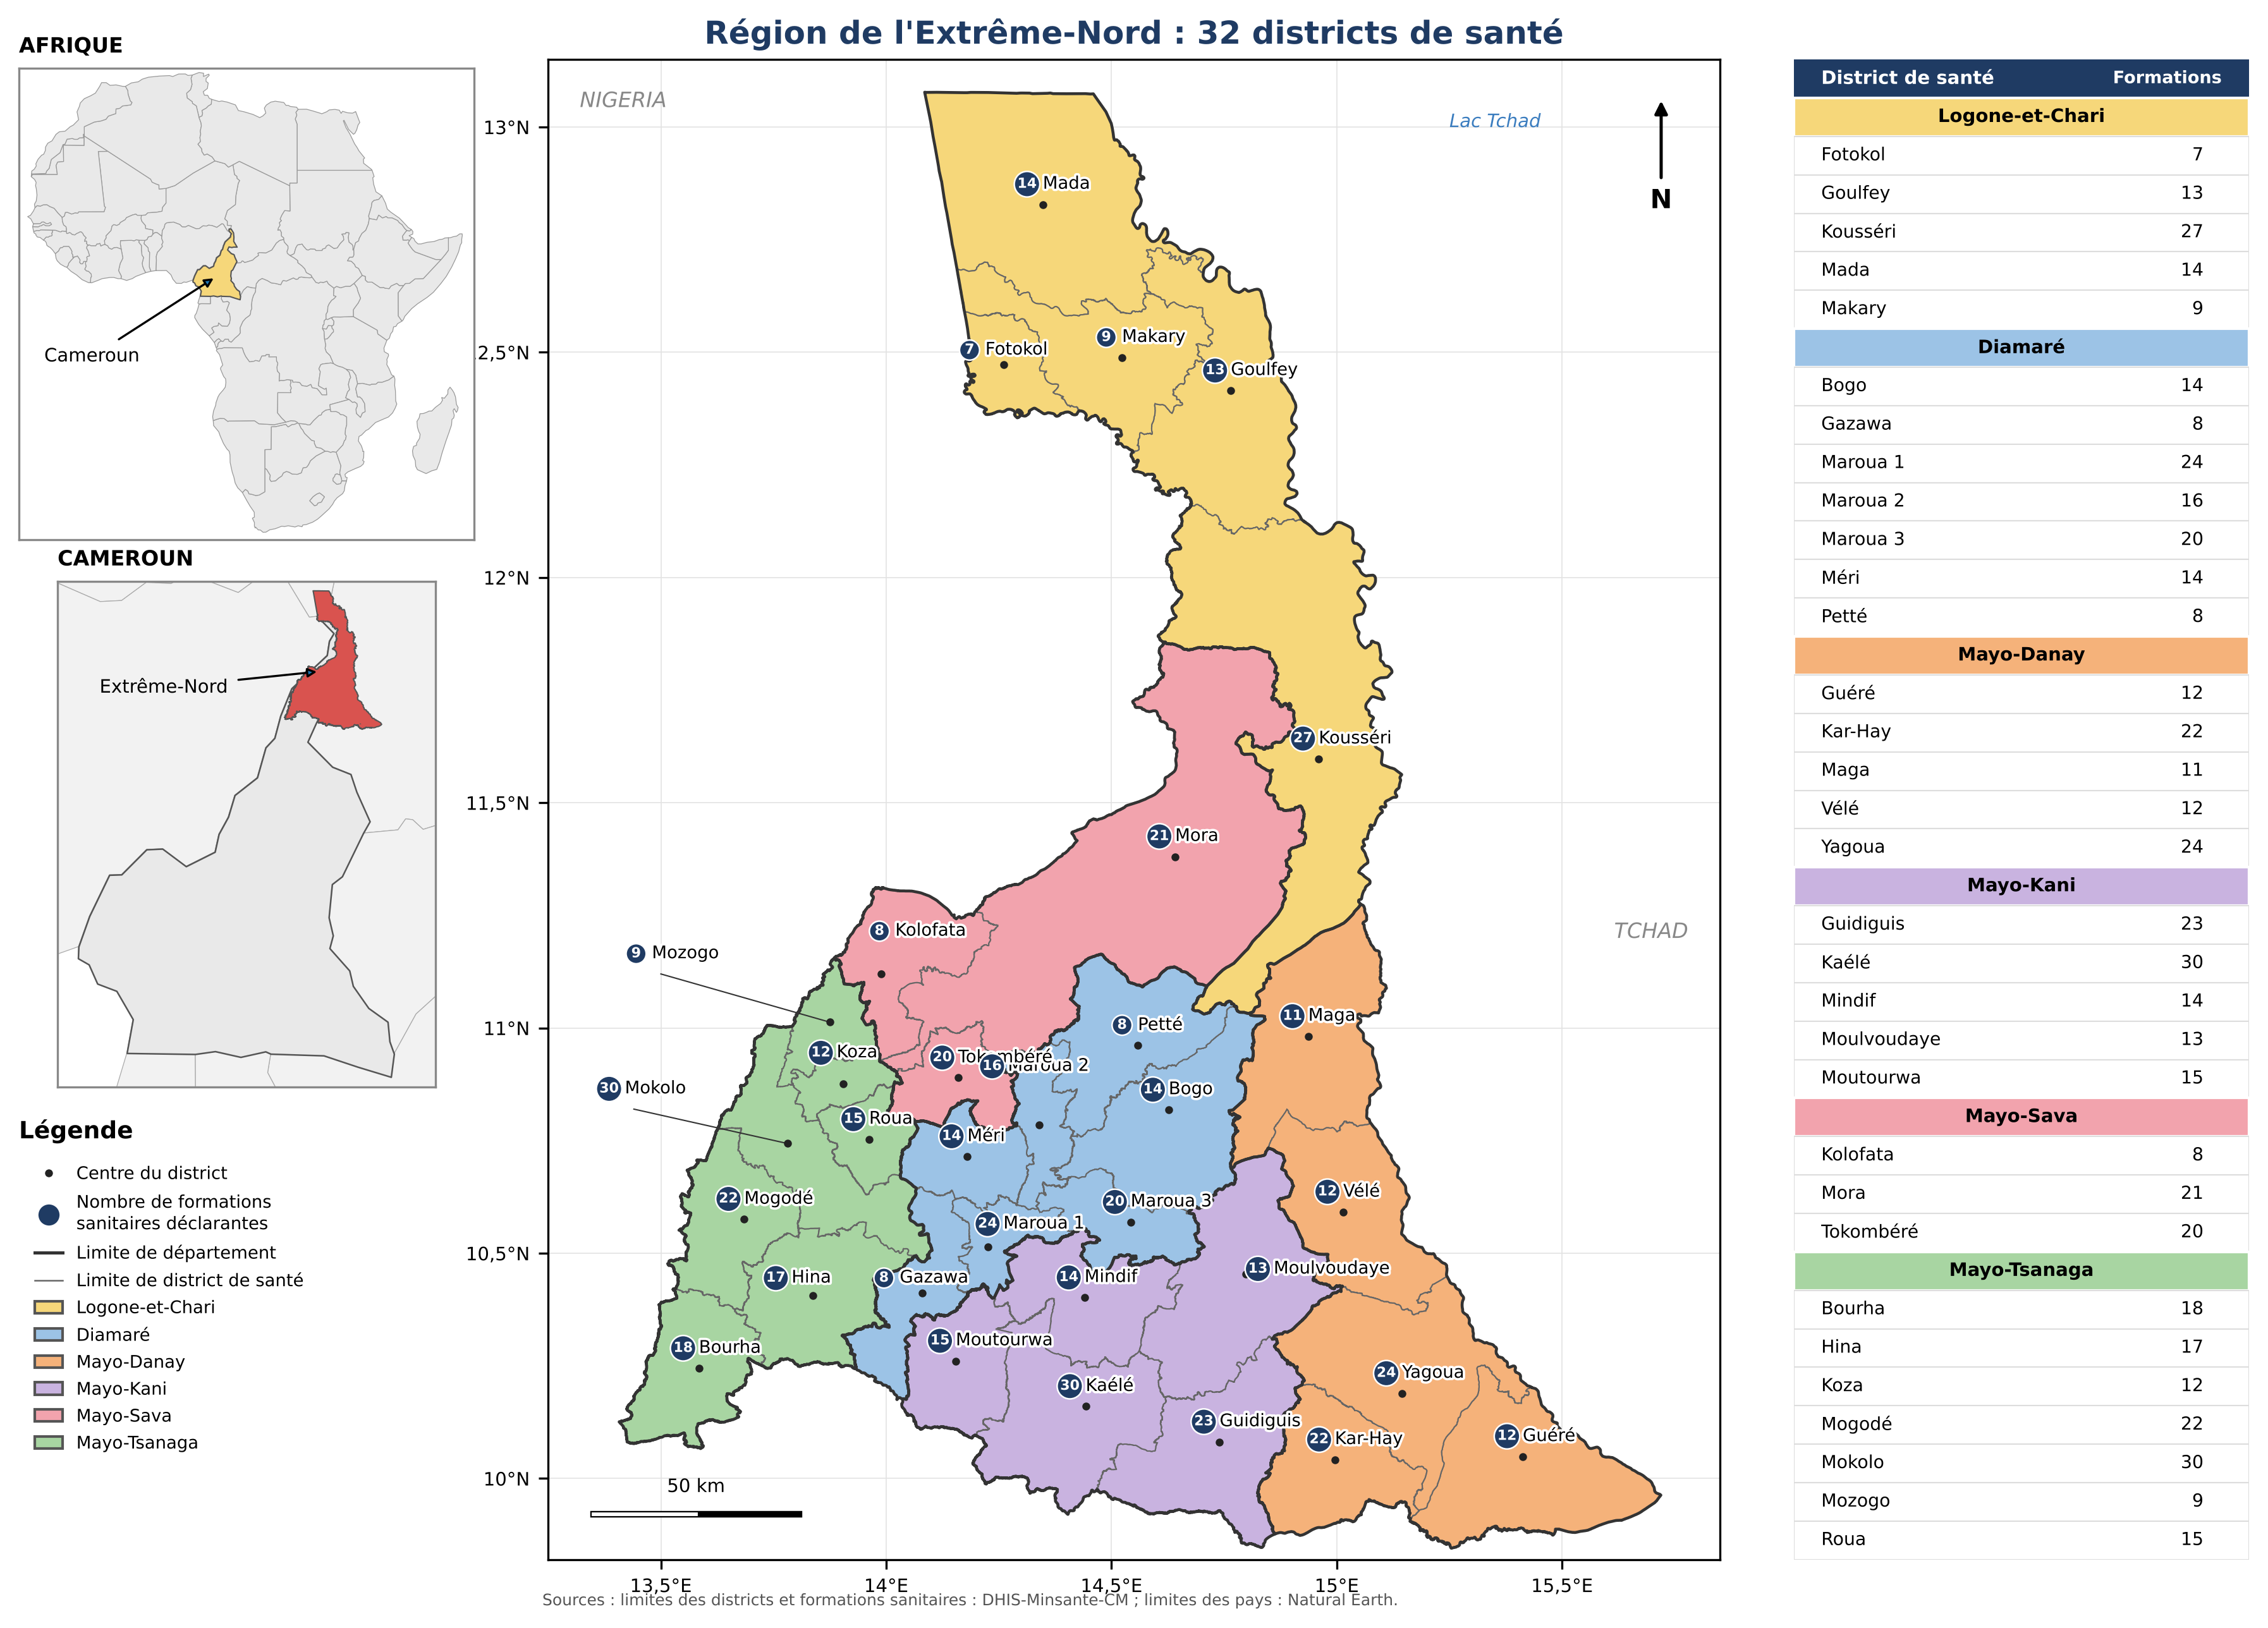
\includegraphics[width=0.95\textheight]{figures/fr_zone_etude.png}\caption{Zone d'étude. À gauche : situation du Cameroun en Afrique et de la région de l'Extrême-Nord au Cameroun, et légende. Au centre : les 32 districts de santé, colorés par département ; le chiffre dans le cercle indique le nombre de formations sanitaires déclarantes du district. À droite : liste des districts par département. Limites des districts et formations sanitaires : DHIS-Minsante-CM ; limites des pays : Natural Earth.}\label{fig:f2a_reference}\end{sidewaysfigure}

\subsection{Sources des données}
Les données de surveillance ont été extraites de DHIS-Minsante-CM (\url{https://dhis-minsante-cm.org}), le système d'information sanitaire national du ministère de la Santé publique, fondé sur la plateforme DHIS2 [\hyperlink{ref4}{4}]. Ce système centralise chaque semaine les cas des maladies sous surveillance déclarés par les formations sanitaires. Les cas hebdomadaires de fièvre typhoïde (élément de données MAPE16\_H\_10) ont été exportés pour les 522 formations sanitaires de la région, de la semaine 1 de 2019 à la semaine 52 de 2025 (365 semaines), en collaboration avec la Délégation régionale de la santé publique de l'Extrême-Nord. Conformément aux protocoles nationaux de routine, et en l'absence d'hémoculture dans les formations sanitaires périphériques, ces cas correspondent principalement à des cas cliniquement suspects confirmés par le sérodiagnostic de Widal [\hyperlink{ref3}{3}]. Les limites des districts et la hiérarchie des formations sanitaires ont été exportées du même système.

Les précipitations corrigées, la température moyenne à 2 m et l'humidité relative quotidiennes ont été obtenues auprès de NASA POWER [\hyperlink{ref11}{11}] pour un point situé à l'intérieur de chaque district, calculé à partir des limites des districts.

\subsection{Prétraitement des données}
Le prétraitement a suivi neuf étapes (tableau~\ref{tab:pretraitement}). Les cas exportés par formation, semaine et catégorie d'âge et de sexe ont été additionnés par district et par semaine, puis harmonisés : les districts créés récemment ont été ramenés à leur district d'origine, et les deux formations aujourd'hui rattachées à Waza ont été réintégrées dans Mora, ce que confirment les données historiques (250 semaines identiques sur 261). L'export a été validé par comparaison avec une extraction antérieure portant sur 2019-2023 (écart médian de 0\,\%).

Une semaine-district sans aucune déclaration a été considérée comme manquante et imputée par interpolation linéaire au sein du district. Les valeurs inhabituelles ont été recherchées par le filtre de Hampel [\hyperlink{ref12}{12}] ; faute de pouvoir distinguer une erreur de saisie d'une flambée réelle, elles ont été conservées. La relation entre la moyenne et la variance des cas des districts, estimée par la loi de Taylor [\hyperlink{ref13}{13}], a justifié l'échelle logarithmique utilisée pour le modèle global. Enfin, la série régionale a été décomposée en tendance, saison et résidu par la méthode STL [\hyperlink{ref14}{14}], sa stationnarité évaluée par les tests de Dickey-Fuller augmenté [\hyperlink{ref15}{15}] et KPSS [\hyperlink{ref16}{16}], et son autocorrélation par la statistique de Ljung-Box [\hyperlink{ref17}{17}]. Les données climatiques quotidiennes ont été agrégées en semaines du lundi au dimanche, alignées sur les semaines épidémiologiques. Les formules de chaque étape sont données dans le matériel supplémentaire S1.

\begin{table}[!htbp]\centering\small
\caption{Étapes du prétraitement des données.}\label{tab:pretraitement}
\begin{tabularx}{\linewidth}{@{}c >{\raggedright\arraybackslash}p{2.5cm} L >{\raggedright\arraybackslash}p{4.2cm}@{}}\toprule
N° & Étape & Opération & Résultat \\\midrule
1 & Extraction & Export DHIS2 brut par formation, semaine, âge et sexe & 617\,481 lignes ; 522 formations \\
2 & Agrégation & Somme par district et par semaine, à l'aide de la hiérarchie & 32 séries de 365 semaines \\
3 & Harmonisation & Réintégration des nouveaux districts (Waza dans Mora) & Découpage constant sur 2019-2025 \\
4 & Validation & Comparaison avec une extraction antérieure (2019-2023) & Écart médian de 0\,\% \\
5 & Données manquantes & Interpolation linéaire au sein de chaque district & 5,5\,\% des semaines-districts imputées \\
6 & Valeurs aberrantes & Filtre de Hampel (fenêtre de 9 semaines, seuil de 3 écarts) & 417 valeurs signalées (3,8\,\%), conservées \\
7 & Climat & Agrégation hebdomadaire des données NASA POWER & Pluie, température et humidité alignées \\
8 & Transformation & $\ln(1+y)$ pour le modèle global (loi de Taylor) & Variance stabilisée entre districts \\
9 & Exploration & STL, ADF, KPSS, ACF/PACF, Ljung-Box & Différenciation d'ordre 1 retenue \\\bottomrule
\end{tabularx}
\end{table}

\subsection{Construction des variables}
Les variables explicatives ont été construites à partir de la seule information disponible à la date de prévision (tableau~\ref{tab:variables}). Elles décrivent les cas récents, la période de l'année et, pour les modèles avec climat, la pluie, la température et l'humidité des semaines précédentes. Le modèle global reçoit en plus le niveau habituel de chaque district.

\begin{table}[!htbp]\centering\small
\caption{Variables utilisées par les modèles XGBoost, avec leur justification.}\label{tab:variables}
\begin{tabularx}{\linewidth}{@{}>{\raggedright\arraybackslash}p{4.4cm} L L@{}}\toprule
Variable & Description & Justification \\\midrule
Cas des semaines $t$ à $t-3$ & Cas déclarés la semaine courante et les trois précédentes & Persistance des cas d'une semaine à l'autre \\
Moyenne sur 4 semaines & Moyenne des cas des 4 dernières semaines & Tendance à court terme, atténue le bruit \\
Moyenne sur 13 semaines & Moyenne des cas des 13 dernières semaines & Tendance trimestrielle \\
Semaine de l'année (sinus, cosinus) & Position de la semaine visée dans l'année & Saisonnalité ; la semaine 52 est voisine de la semaine 1 \\
Même semaine l'année précédente & Cas de la semaine visée, un an plus tôt & Mémoire de la saison précédente \\
Niveau du district (modèle global) & Moyenne passée de $\ln(1+y)$ du district & Adapte le modèle commun à la taille du district \\
Pluie cumulée sur 4 semaines & Pluie des semaines $t$ à $t-3$ & Effet récent de la pluie \\
Pluie cumulée décalée de 4 semaines & Pluie des semaines $t-4$ à $t-7$ & Effet retardé de la pluie (contamination de l'eau) \\
Température et humidité sur 4 semaines & Moyennes des 4 dernières semaines & Conditions de survie des bactéries \\\bottomrule
\end{tabularx}
\par\smallskip\footnotesize\raggedright Les variables climatiques ne sont utilisées que par le modèle « XGBoost avec climat ».
\end{table}

\subsection{Étapes de l'étude}
La figure~\ref{fig:pipeline2} résume les étapes suivies, regroupées en cinq phases. Les données de surveillance, de climat et de découpage ont d'abord été collectées (phase 1), puis agrégées, contrôlées et transformées (phase 2). La série a ensuite été explorée, le modèle mathématique a servi à formuler les hypothèses, et les variables explicatives ont été construites (phase 3). Les méthodes de prévision ont été évaluées par origine glissante et comparées statistiquement (phase 4), avant la traduction des résultats en recommandations (phase 5).

\begin{figure}[!htbp]\centering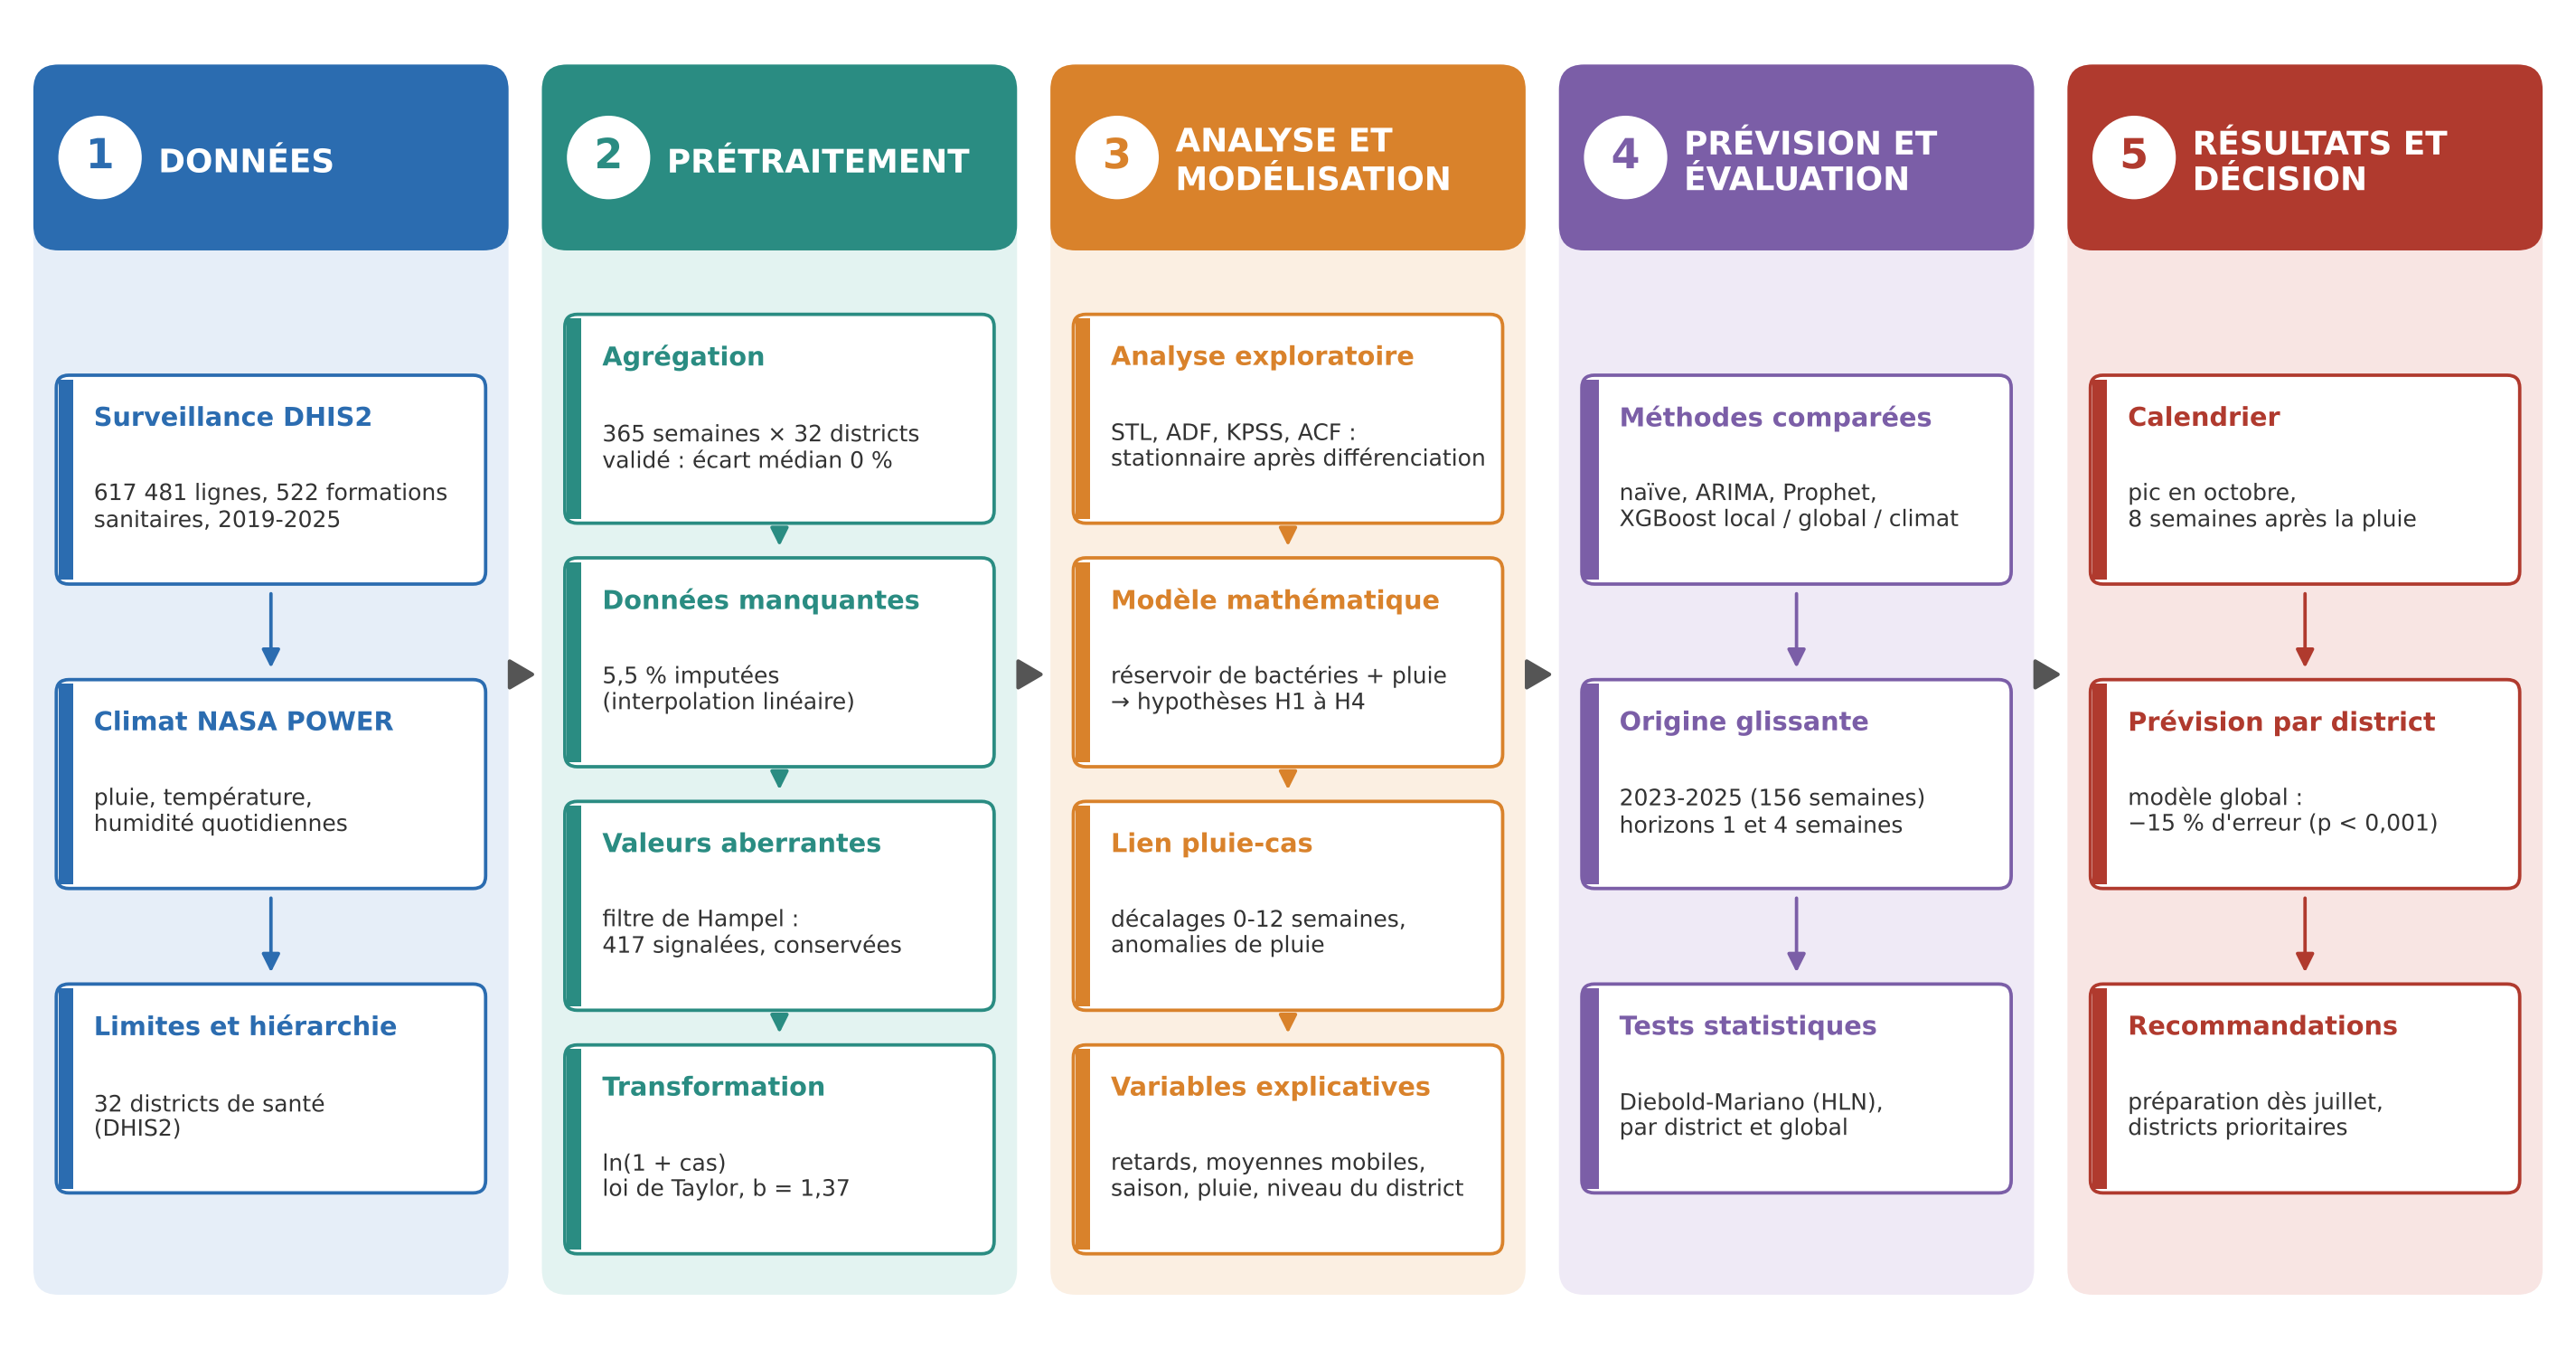
\includegraphics[width=\linewidth]{figures/fr_etapes.png}\caption{Étapes suivies dans l'étude, de la collecte des données à l'aide à la décision.}\label{fig:pipeline2}\end{figure}

\subsection{Cadre de modélisation mathématique}
Nous sommes partis d'un modèle de transmission de la typhoïde à réservoir environnemental [\hyperlink{ref5}{5},\hyperlink{ref6}{6}] (figure~\ref{fig:schema_modele}). La population est répartie entre personnes sensibles, porteurs sans symptômes, malades et guéris ; les porteurs et les malades rejettent des bactéries qui s'accumulent dans l'eau et les aliments. Le risque d'infection d'une personne sensible, ou force d'infection $\lambda$, dépend de la concentration de bactéries $B$ selon une loi saturante :
\begin{equation}
\lambda(t)=\frac{\nu\,B(t)}{K+B(t)} ,
\label{eq:lambda}
\end{equation}
où $\nu$ est le risque maximal et $K$ la concentration à laquelle ce risque atteint la moitié de son maximum. Nous avons ajouté au modèle l'effet de la pluie $P(t)$, qui accroît la contamination de l'environnement avec une intensité $\kappa$, tandis que les bactéries disparaissent au taux $\mu_b$ :
\begin{equation}
\frac{dB}{dt}=\sigma_1 C+\sigma_2 I+\kappa\,P(t)-\mu_b B ,
\label{eq:pluie}
\end{equation}
où $C$ et $I$ sont les porteurs et les malades, et $\sigma_1$, $\sigma_2$ leurs taux de rejet de bactéries.

\fig{schema_modele}{0.85}{Modèle de transmission de la fièvre typhoïde avec réservoir environnemental et effet de la pluie. S : sensibles ; C : porteurs ; I : malades ; R : guéris ; B : bactéries dans l'eau et les aliments. Les paramètres sont définis dans le matériel supplémentaire S1.}

Ce modèle conduit à deux prédictions testables. D'abord, la pluie n'agit pas immédiatement : elle doit d'abord contaminer le réservoir, puis l'infection doit incuber (environ 6 à 30 jours [\hyperlink{ref6}{6}]) avant la consultation et la déclaration ; le pic des cas devrait donc suivre celui des pluies de plusieurs semaines. Ensuite, la loi~\eqref{eq:lambda} sature : lorsque l'environnement est déjà très contaminé, un surplus de pluie n'augmente presque plus le risque ; une saison plus pluvieuse que la normale pourrait alors ne pas donner davantage de cas. Les paramètres n'étant pas connus pour l'Extrême-Nord, le modèle n'a pas été ajusté : il a servi à formuler ces hypothèses, testées sur les données.

\subsection{Lien entre pluie et cas}
Pour isoler la saisonnalité de la tendance liée à l'extension du réseau, les cas de chaque semaine ont été rapportés à leur moyenne sur les 52 semaines environnantes. Ces cas « sans tendance » ont été corrélés à la pluie cumulée des 4 semaines précédentes, pour des décalages de 0 à 12 semaines. Pour distinguer le calendrier de l'intensité, l'analyse a été répétée avec l'anomalie de pluie, c'est-à-dire l'écart à la pluie habituelle de la même semaine de l'année. Des indices saisonniers mensuels ont aussi été calculés, selon une démarche proche de celle de Shashvat et al. [\hyperlink{ref7}{7}]. Les analyses ont été conduites pour la région et pour chaque district ; les associations entre caractéristiques des districts ont été testées par corrélation de Spearman.

\subsection{Prévision des cas et évaluation}
Nous avons comparé la méthode de référence dite « naïve », qui reconduit la valeur de la semaine courante ; la même semaine de l'année précédente ; le modèle statistique ARIMA [\hyperlink{ref18}{18}] ; Prophet [\hyperlink{ref19}{19}] ; et XGBoost [\hyperlink{ref20}{20}], avec et sans variables climatiques (tableau~\ref{tab:hyper}). Au niveau des districts, nous avons comparé des modèles ajustés district par district à un modèle unique entraîné sur les 32 districts à la fois, dit modèle global [\hyperlink{ref21}{21},\hyperlink{ref22}{22}]. Ce modèle prédit la variation relative des cas de chaque district $d$ à l'horizon de $h$ semaines :
\begin{equation}
\ln(1+y_{d,t+h})-\ln(1+y_{d,t})=F_h\big(\mathbf{x}_{d,t},\,\bar{u}_{d,t}\big)+\varepsilon_{d,t+h} ,
\label{eq:global}
\end{equation}
où $y_{d,t}$ est le nombre de cas, $\mathbf{x}_{d,t}$ les variables du tableau~\ref{tab:variables}, $\bar{u}_{d,t}$ le niveau habituel du district, et $F_h$ une seule fonction apprise sur tous les districts.

\begin{table}[!htbp]\centering\small
\caption{Spécification des méthodes de prévision.}\label{tab:hyper}
\begin{tabularx}{\linewidth}{@{}>{\raggedright\arraybackslash}p{3.6cm} L L@{}}\toprule
Méthode & Spécification & Paramètres \\\midrule
Naïve ; même semaine l'année précédente & Reconduction de la dernière valeur ; valeur un an plus tôt & Aucun \\
ARIMA & Ordre choisi sur 2019-2022 (KPSS, critère d'Akaike), puis figé & Régional : ARIMA(2,1,1) ; un ordre par district \\
Prophet & Tendance par morceaux et saisonnalité annuelle & Série de Fourier d'ordre 10 \\
XGBoost (local, global, avec climat) & Un modèle par horizon ; prévoit la variation des cas & 300 arbres ; profondeur 3 ; taux 0,05 ; sous-échantillonnage 0,8 \\\bottomrule
\end{tabularx}
\par\smallskip\footnotesize\raggedright Les réglages ont été fixés avant l'évaluation et jamais ajustés sur la période test.
\end{table}

Les prévisions à 1 et 4 semaines ont été évaluées sur 2023-2025 (156 semaines), période où le réseau de surveillance était stable. Chaque semaine, chaque modèle était réentraîné sur les seules données passées, comme en situation réelle (origine glissante [\hyperlink{ref23}{23}]). La précision a été mesurée par l'erreur absolue moyenne (MAE) [\hyperlink{ref24}{24}], la racine de l'erreur quadratique moyenne (RMSE) et l'erreur en pourcentage (MAPE). Les différences entre méthodes ont été testées par le test de Diebold-Mariano [\hyperlink{ref25}{25}] avec la correction de Harvey, Leybourne et Newbold [\hyperlink{ref26}{26}], district par district et pour l'ensemble des districts. L'évaluation régionale a été répétée en excluant les districts à données incomplètes.

\subsection{Logiciels et éthique}
Les analyses ont été réalisées en Python (pandas, statsmodels, prophet, xgboost, scipy) ; les scripts d'analyse sont déposés dans un dépôt GitHub public (typhoide-extreme-nord). L'étude n'utilise que des données agrégées de surveillance de routine, sans information individuelle ; leur utilisation a été autorisée par la Délégation régionale de la santé publique de l'Extrême-Nord (DRSP-EN).

\section{Résultats}
\subsection{Description des données}
Entre 2019 et 2025, 417\,910 cas ont été déclarés, soit 1\,145 par semaine en moyenne (tableau~\ref{tab:desc}, figure~\ref{fig:f3_serie}). Les cas étaient concentrés dans les districts urbains et frontaliers : Kousséri (13,9\,\%), Maroua 1 (11,0\,\%), Mokolo (10,0\,\%), Mora (5,7\,\%) et Yagoua (5,4\,\%) (figure~\ref{fig:cartes}A). La hausse des cas déclarés entre 2019 et 2022 coïncidait avec l'extension du réseau : le nombre de formations déclarantes a triplé, puis s'est stabilisé autour de 360 (tableau~\ref{tab:fac}). Sur la période stable 2022-2025, les cas n'ont augmenté que de 20\,\%.

\begin{table}[!htbp]\centering\small
\caption{Statistiques descriptives des cas hebdomadaires déclarés, Extrême-Nord, 2019-2025.}\label{tab:desc}
\begin{tabularx}{\linewidth}{@{}L r@{}}\toprule
Indicateur & Valeur \\\midrule
Semaines × districts & 365 × 32 \\
Total des cas déclarés & 417\,910 \\
Cas par semaine (région) : moyenne (écart-type) & 1\,145 (315) \\
Cas par semaine (région) : médiane [Q1 ; Q3] & 1\,143 [969 ; 1\,340] \\
Cas par semaine (région) : minimum ; maximum & 328 (juin 2019) ; 1\,956 (sept. 2025) \\
Cas moyens par semaine et par district : médiane [min ; max] & 29,3 [2,2 ; 159,7] \\
Semaines-districts manquantes & 5,5\,\% \\
Valeurs aberrantes signalées (filtre de Hampel) & 417 (3,8\,\%) \\\bottomrule
\end{tabularx}
\end{table}

\begin{table}[!htbp]\centering\small
\caption{Formations sanitaires déclarantes, cas hebdomadaires moyens et pluie annuelle, Extrême-Nord.}\label{tab:fac}
\begin{tabular}{@{}lrrrrrrr@{}}\toprule
 & 2019 & 2020 & 2021 & 2022 & 2023 & 2024 & 2025 \\\midrule
Formations déclarantes (moyenne/semaine) & 104 & 145 & 231 & 334 & 358 & 359 & 364 \\
Cas par semaine (moyenne régionale) & 689 & 950 & 1\,147 & 1\,188 & 1\,258 & 1\,371 & 1\,425 \\
Semaines-districts manquantes (\%) & 20,3 & 11,2 & 3,4 & 0,0 & 1,1 & 0,9 & 1,1 \\
Pluie annuelle (mm, moyenne régionale) & 829 & 627 & 545 & 822 & 623 & 832 & 748 \\\bottomrule
\end{tabular}
\end{table}

\fig{f3_serie}{0.95}{Cas hebdomadaires de fièvre typhoïde déclarés dans l'Extrême-Nord (trait plein) et nombre de formations sanitaires déclarantes (tirets), 2019-2025. La zone colorée indique la période d'évaluation des prévisions.}

\begin{figure}[!htbp]\centering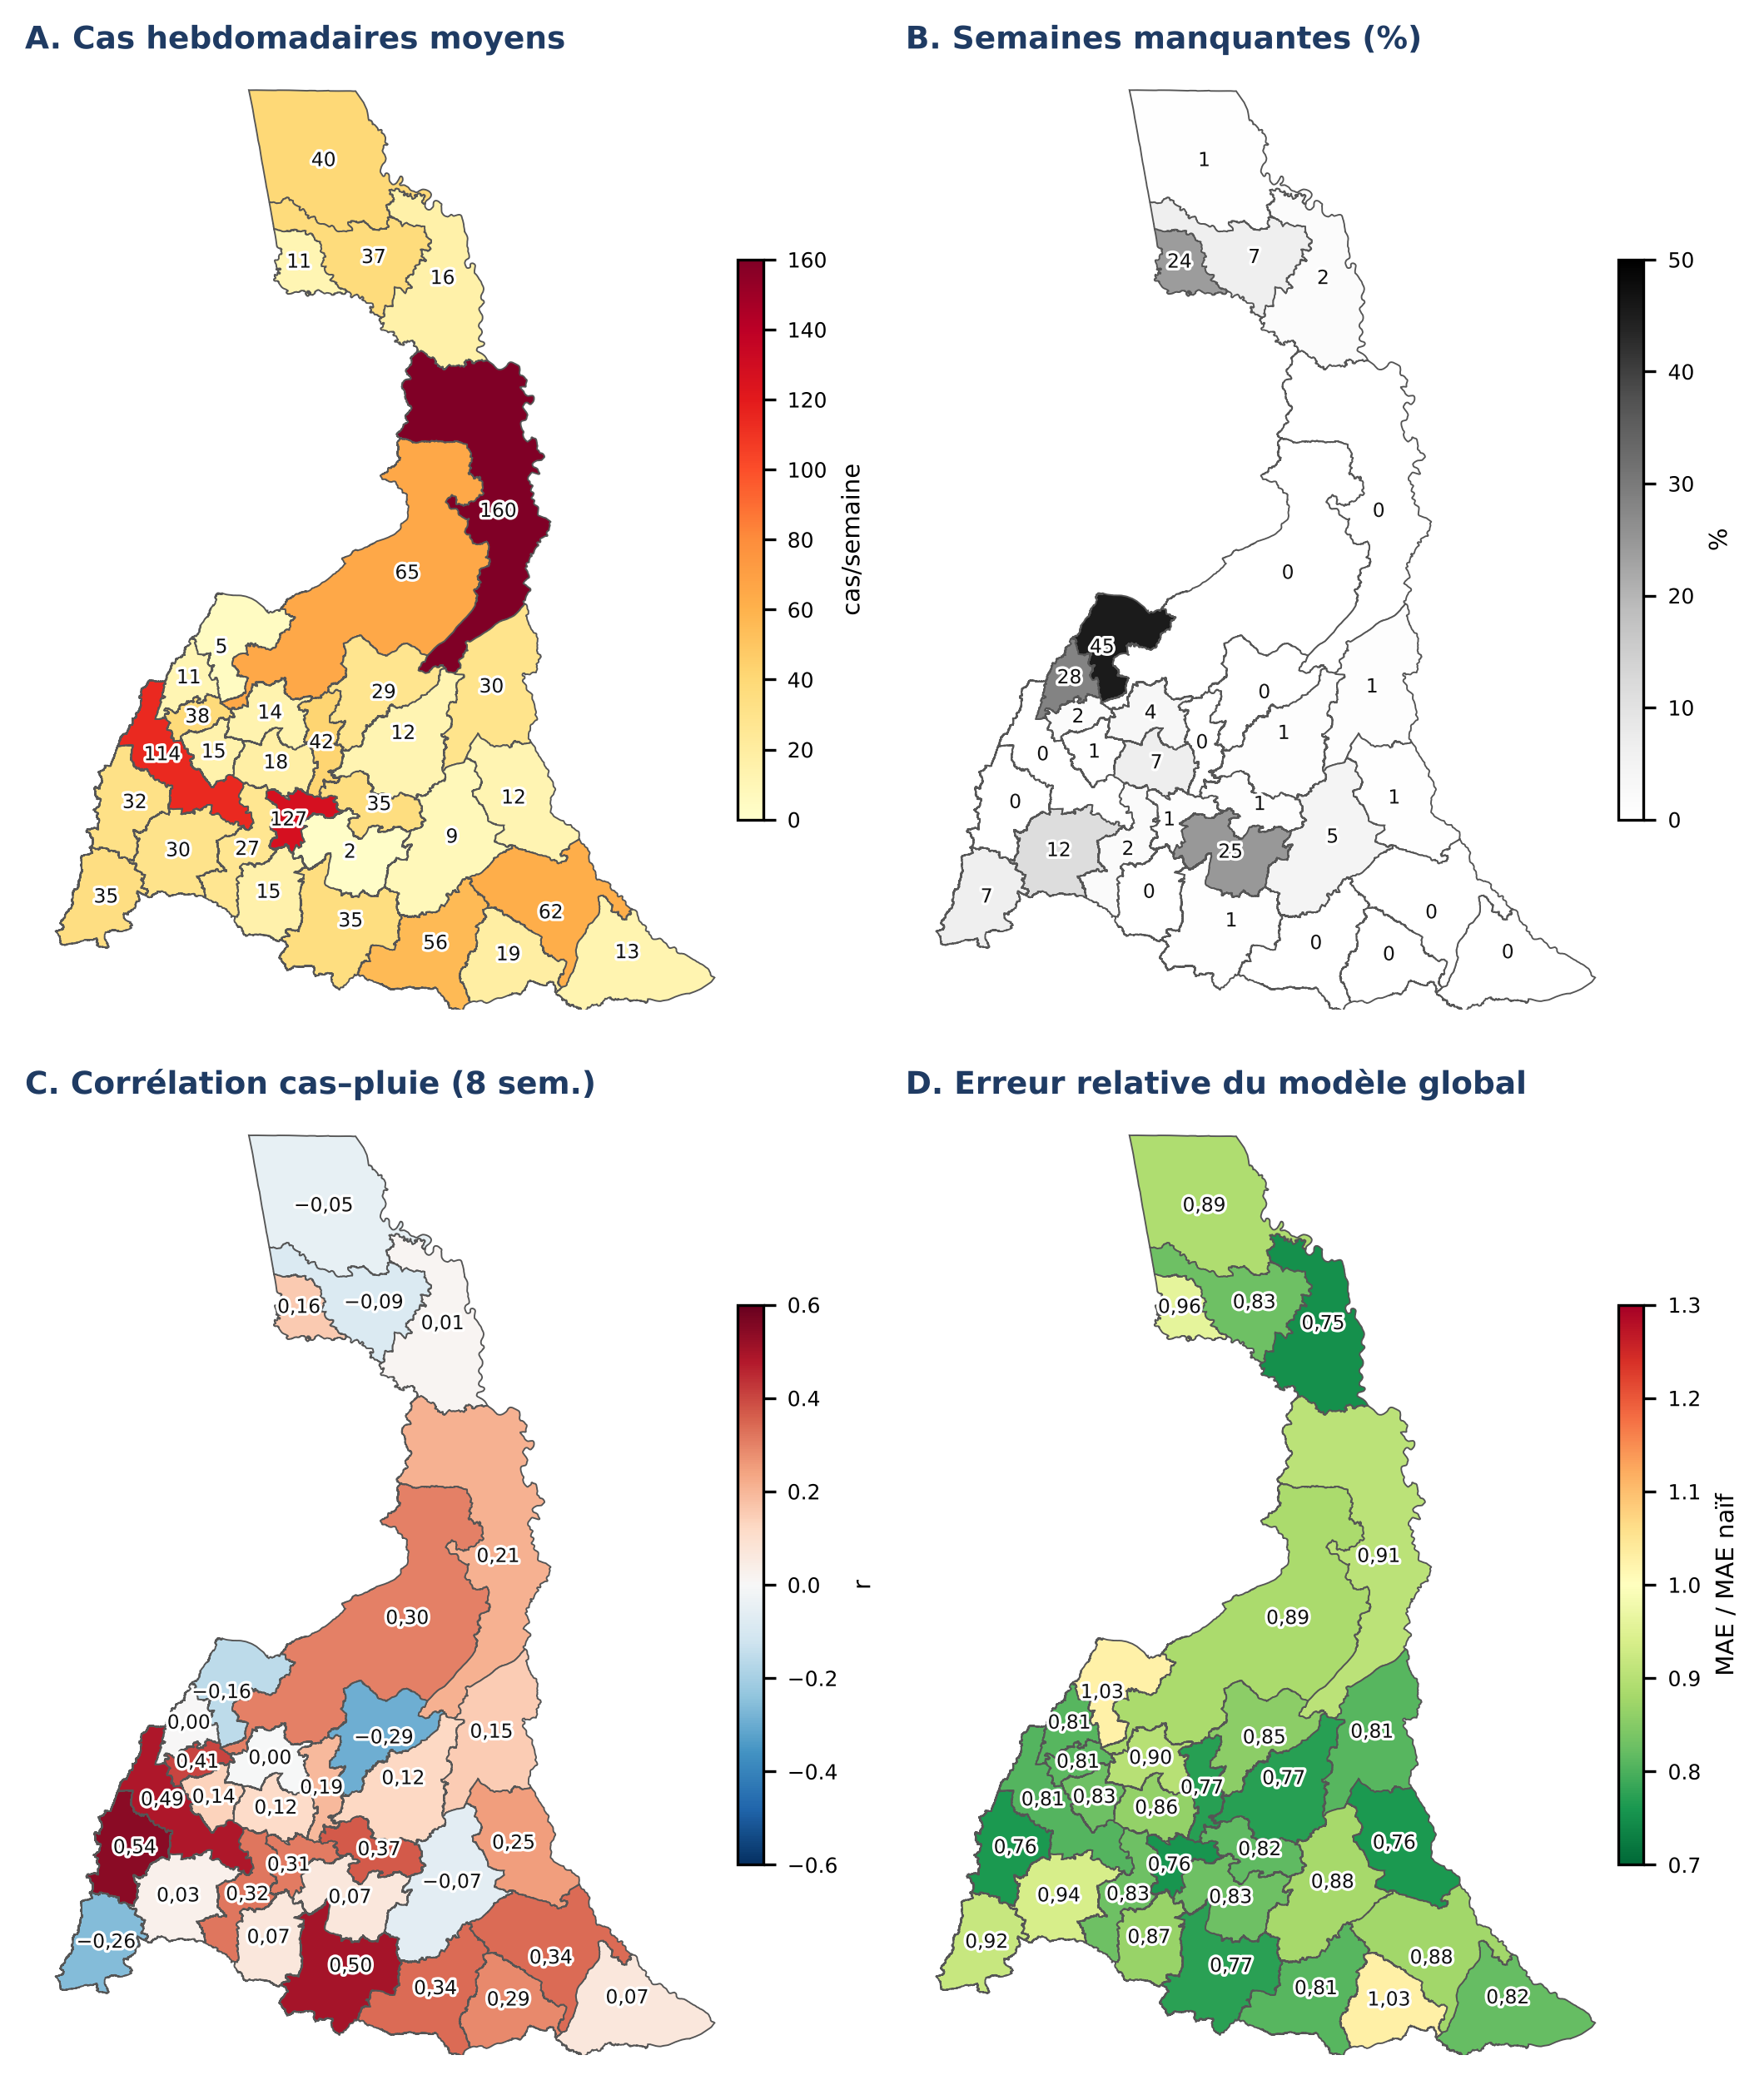
\includegraphics[width=0.92\linewidth]{figures/fr_cartes_composite.png}\caption{Résultats par district de santé : (A) cas hebdomadaires moyens ; (B) part des semaines manquantes ; (C) corrélation entre cas et pluie à 8 semaines de décalage ; (D) erreur du modèle global rapportée à celle de la méthode naïve, à 4 semaines (inférieure à 1 : meilleur). Les noms des districts figurent sur la figure~\ref{fig:f2a_reference} et les valeurs détaillées à l'annexe A.}\label{fig:cartes}\end{figure}

\subsection{Qualité des données et structure de la série}
Les données manquantes étaient concentrées au début de la période (20,3\,\% des semaines-districts en 2019, moins de 1,2\,\% à partir de 2022) et dans quatre districts, dont plusieurs sont touchés par l'insécurité : Kolofata (45,5\,\%), Mozogo (28,5\,\%), Mindif (24,7\,\%) et Fotokol (24,1\,\%) (figures~\ref{fig:cartes}B et~\ref{fig:f4_manquants}). Les 417 valeurs inhabituelles signalées étaient réparties sur toute l'année. La loi de Taylor donnait un exposant de 1,37 : la variabilité des cas croît plus vite que leur niveau, ce qui justifie l'échelle logarithmique du modèle global.

\fig{f4_manquants}{0.92}{Structure des semaines manquantes par district (lignes, triées par part décroissante) et par semaine (colonnes).}

La décomposition de la série régionale faisait apparaître une tendance croissante jusqu'en 2022, liée à l'extension du réseau, et une saison annuelle régulière, avec un pic chaque année entre septembre et novembre (figure~\ref{fig:f5_stl}) ; la force de la tendance était de 0,77 et celle de la saison de 0,57. La série n'était pas stationnaire en niveau, mais le devenait après différenciation d'une semaine à l'autre (tableau~\ref{tab:stat}). Les cas d'une semaine étaient fortement liés à ceux des semaines précédentes, avec une remontée vers 52 semaines traduisant la saisonnalité annuelle (figure~\ref{fig:f7_acf} ; Ljung-Box, $p<0{,}001$). Le modèle ARIMA(2,1,1) laissait des résidus non autocorrélés ($p=0{,}71$ à 4 semaines). Ces résultats ont guidé le choix des modèles : prévoir la variation des cas plutôt que leur niveau, et tenir compte de la période de l'année.

\fig{f5_stl}{0.9}{Décomposition de la série régionale hebdomadaire en tendance, saison et résidu (méthode STL, période de 52 semaines).}

\begin{table}[!htbp]\centering\small
\caption{Tests de stationnarité de la série régionale hebdomadaire, 2019-2025.}\label{tab:stat}
\begin{tabularx}{\linewidth}{@{}L rrrr L@{}}\toprule
Transformation & ADF & $p$ (ADF) & KPSS & $p$ (KPSS) & Conclusion \\\midrule
Niveau & $-3{,}22$ & 0,019 & 2,13 & $<0{,}01$ & Non stationnaire (tendance) \\
Logarithme & $-3{,}21$ & 0,019 & 2,09 & $<0{,}01$ & Non stationnaire (tendance) \\
Différence première & $-26{,}11$ & $<0{,}001$ & 0,06 & $>0{,}10$ & Stationnaire \\
Différence saisonnière (52) & $-4{,}43$ & $<0{,}001$ & 0,37 & 0,09 & Stationnaire \\\bottomrule
\end{tabularx}
\par\smallskip\footnotesize\raggedright ADF : l'hypothèse nulle est la non-stationnarité ; KPSS : l'hypothèse nulle est la stationnarité.
\end{table}

\fig{f7_acf}{0.9}{Autocorrélation (ACF) et autocorrélation partielle (PACF) de la série régionale, en niveau et après différenciation. La bande grise indique l'intervalle de confiance à 95\,\%.}

\subsection{La pluie fixe le calendrier de la saison}
La saison de typhoïde suivait régulièrement la saison des pluies (figure~\ref{fig:f6_indices}). Juin à septembre concentraient 88\,\% des précipitations, avec un pic en août. Rapportés à leur tendance, les cas étaient au plus bas en juin (16\,\% sous la normale) et au plus haut en octobre (24\,\% au-dessus), soit environ deux mois après le pic des pluies. La corrélation entre les cas sans tendance et la pluie des semaines précédentes croissait avec le décalage et culminait à 0,54 pour 8 semaines (figure~\ref{fig:f8_correlation}), comme prévu par le modèle.

\fig{f6_indices}{0.85}{Indices saisonniers mensuels des cas de typhoïde (courbe ; 1 = niveau moyen de l'année) et répartition mensuelle des précipitations (barres), Extrême-Nord, 2019-2025.}

\fig{f8_correlation}{0.88}{Corrélation entre les cas hebdomadaires sans tendance et la pluie cumulée des 4 semaines précédentes (bleu) ou son anomalie par rapport à la normale (orange), selon le décalage en semaines. La bande grise indique le seuil de significativité à 5\,\%.}

Le lien était net (corrélation d'au moins 0,30) dans 10 districts, surtout dans le sud-ouest et le centre de la région : Mogodé (0,54), Kaélé (0,50), Mokolo (0,49), Koza (0,41), Maroua 3 (0,37), Guidiguis (0,34), Yagoua (0,34), Gazawa (0,32), Maroua 1 (0,31) et Mora (0,30) (figure~\ref{fig:cartes}C). Il était plus fort dans les districts qui déclaraient le plus de cas ($\rho=0{,}49$ ; $p=0{,}004$) et dont les données étaient les plus complètes ($\rho=-0{,}48$ ; $p=0{,}005$).

\subsection{La pluie ne fixe pas l'intensité des pics}
Une saison plus pluvieuse que la normale n'entraînait pas davantage de cas : la corrélation avec l'anomalie de pluie était même légèrement négative ($r=-0{,}19$ à 8 semaines ; figure~\ref{fig:f8_correlation}), et aucun district ne présentait d'association positive notable. L'année 2023, l'une des moins pluvieuses (623 mm), a ainsi connu l'un des pics les plus marqués de la période (tableau~\ref{tab:fac}, figure~\ref{fig:f3_serie}).

\subsection{Prévisions régionales}
Au niveau régional, aucune méthode ne prévoyait significativement mieux que la méthode naïve, à 1 comme à 4 semaines (tableau~\ref{tab:reg}). L'ajout des variables de pluie, de température et d'humidité n'améliorait pas la précision de XGBoost ($p=0{,}31$ à 1 semaine ; $p=0{,}77$ à 4 semaines). Tous les modèles suivaient les pics avec retard (figure~\ref{fig:f10_previsions}).

\begin{table}[!htbp]\centering\small
\caption{Précision des prévisions régionales, 2023-2025 (156 semaines à 1 semaine, 153 à 4 semaines). MAE et RMSE en cas par semaine.}\label{tab:reg}
\begin{tabular}{@{}llrrrrl@{}}\toprule
Horizon & Méthode & MAE & RMSE & MAPE (\%) & Gain vs naïve (\%) & $p$ \\\midrule
\multirow{6}{*}{1 semaine} & ARIMA & 102,3 & 127,5 & 7,6 & +4,7 & 0,15 \\
 & XGBoost & 105,4 & 135,8 & 7,7 & +1,8 & 0,68 \\
 & Naïve (référence) & 107,3 & 135,2 & 7,9 & -- & -- \\
 & XGBoost avec climat & 108,5 & 141,2 & 7,9 & $-1{,}1$ & 0,80 \\
 & Prophet & 132,3 & 174,9 & 9,4 & $-23{,}3$ & 0,013\,$^{\dagger}$ \\
 & Même semaine an passé & 208,9 & 271,0 & 14,8 & $-94{,}7$ & $<0{,}001$\,$^{\dagger}$ \\\midrule
\multirow{6}{*}{4 semaines} & XGBoost avec climat & 142,4 & 192,5 & 10,3 & +10,7 & 0,15 \\
 & XGBoost & 143,9 & 189,7 & 10,3 & +9,8 & 0,22 \\
 & Prophet & 145,5 & 195,2 & 10,2 & +8,8 & 0,48 \\
 & ARIMA & 153,8 & 203,0 & 11,1 & +3,6 & 0,41 \\
 & Naïve (référence) & 159,5 & 211,9 & 11,6 & -- & -- \\
 & Même semaine an passé & 210,9 & 273,1 & 14,9 & $-32{,}2$ & 0,06 \\\bottomrule
\end{tabular}
\par\smallskip\footnotesize\raggedright Test de Diebold-Mariano. $^{\dagger}$ Significativement moins précis que la méthode naïve.
\end{table}

\fig{f10_previsions}{0.95}{Prévisions régionales à 4 semaines, 2023-2025 : cas observés et prévisions des principales méthodes.}

\subsection{Prévisions par district}
À l'échelle des districts, le modèle global était le plus précis (tableau~\ref{tab:dist}, figure~\ref{fig:f11_districts}). Sur l'ensemble des districts, il réduisait l'erreur de 13\,\% à 1 semaine et de 15\,\% à 4 semaines par rapport à la méthode naïve ($p<0{,}001$), et de 2 à 5\,\% par rapport à ARIMA ($p=0{,}001$ et $0{,}005$). Il ne faisait significativement moins bien que la méthode naïve dans aucun district ; seuls Kar Hay et Kolofata n'étaient pas mieux prévus (figure~\ref{fig:cartes}D). Les modèles ajustés district par district, faute de données suffisantes, ne faisaient guère mieux que la méthode naïve.

\begin{table}[!htbp]\centering\small
\caption{Précision des prévisions par district, 32 districts, 2023-2025.}\label{tab:dist}
\begin{tabularx}{\linewidth}{@{}l >{\raggedright\arraybackslash}p{3.6cm} R R R@{}}\toprule
Horizon & Méthode & Erreur relative médiane (naïve = 1) & Districts mieux prévus que par la méthode naïve & Significativement meilleurs / moins bons \\\midrule
\multirow{4}{*}{1 semaine} & Modèle global & 0,87 & 31 & 27 / 0 \\
 & ARIMA par district & 0,88 & 30 & 17 / 1 \\
 & XGBoost par district & 0,98 & 21 & 2 / 1 \\
 & Même semaine an passé & 1,44 & 1 & 0 / 29 \\\midrule
\multirow{4}{*}{4 semaines} & Modèle global & 0,83 & 30 & 21 / 0 \\
 & ARIMA par district & 0,89 & 30 & 16 / 1 \\
 & XGBoost par district & 0,96 & 18 & 4 / 0 \\
 & Même semaine an passé & 1,24 & 3 & 0 / 14 \\\bottomrule
\end{tabularx}
\end{table}

\fig{f11_districts}{0.82}{Erreur relative à la méthode naïve, par district et par méthode, à 4 semaines. Les districts sont triés selon l'erreur du modèle global ; une valeur inférieure à 1 indique un gain.}

Pour prévoir, le modèle global s'appuyait d'abord sur les cas de la semaine courante (19,5\,\% de l'importance), la moyenne des 13 dernières semaines (12,1\,\%), les cas de la semaine précédente et le niveau habituel du district (11,1\,\% chacun) ; la période de l'année et la même semaine de l'année précédente représentaient ensemble 21,4\,\% (figure~\ref{fig:f12_importance}).

\fig{f12_importance}{0.82}{Importance relative des variables du modèle global pour la prévision à 4 semaines.}

\subsection{Analyses de sensibilité}
Les conclusions régionales restaient inchangées après exclusion des districts à données incomplètes (tableau~\ref{tab:sens}). Le décalage entre pluie et cas était identique dans tous les scénarios. Le gain de XGBoost était plus marqué avec les seuls districts aux données complètes, et devenait alors à la limite de la significativité ; compte tenu du nombre de comparaisons, ce résultat doit être interprété avec prudence.

\begin{table}[!htbp]\centering\small
\caption{Analyses de sensibilité : prévisions régionales à 4 semaines selon les districts inclus.}\label{tab:sens}
\begin{tabularx}{\linewidth}{@{}L r r r r r r@{}}\toprule
Districts inclus & $n$ & XGBoost (\%) & $p$ & Avec climat (\%) & ARIMA (\%) & $r$ pluie \\\midrule
Tous & 32 & +9,8 & 0,22 & +10,7 & +3,6 & 0,42 \\
Moins de 20\,\% de semaines manquantes & 28 & +8,8 & 0,27 & +10,5 & +3,4 & 0,42 \\
Moins de 5\,\% de semaines manquantes & 24 & +16,4 & 0,053 & +16,2 & $-0{,}6$ & 0,47 \\
Aucune semaine manquante & 9 & +12,3 & 0,044 & +15,2 & +4,3 & 0,43 \\\bottomrule
\end{tabularx}
\par\smallskip\footnotesize\raggedright Gains en réduction de la MAE par rapport à la méthode naïve ; $r$ : corrélation pluie-cas à 8 semaines, sur les séries brutes.
\end{table}

\section{Discussion}
Dans l'Extrême-Nord du Cameroun, la pluie fixe le calendrier de la saison de fièvre typhoïde, mais non son intensité. Le pic des cas survient chaque année en octobre, environ deux mois après le pic des pluies, alors qu'une saison plus pluvieuse que la normale n'entraîne pas davantage de cas et que la pluie n'améliore pas la prévision à court terme.

\subsection{Ce que le modèle mathématique explique}
Ces deux résultats correspondent aux deux prédictions du modèle de transmission. Le décalage de deux mois est compatible avec la chaîne décrite par l'équation~\eqref{eq:pluie} : contamination progressive des puits et des mares au fil de la saison des pluies, incubation, puis consultation et déclaration. Au Népal, les cas suivent aussi la mousson, avec un décalage d'environ un mois après les inondations [\hyperlink{ref9}{9}] ; le décalage plus long observé ici pourrait refléter le contexte sahélien, où les sources d'eau se contaminent progressivement [\hyperlink{ref27}{27}]. La saturation de la force d'infection~\eqref{eq:lambda} offre, elle, une explication à l'absence d'effet de l'intensité des pluies : pendant la saison des pluies, l'environnement serait déjà assez contaminé pour qu'un surplus de pluie ne change presque plus le risque. L'intensité des pics dépendrait alors d'autres facteurs, comme l'accès à l'eau potable, l'assainissement, les déplacements de population ou les pratiques diagnostiques. Cette explication reste une hypothèse, que des mesures de la qualité de l'eau permettraient de tester.

Ce mécanisme explique aussi pourquoi la pluie n'améliore pas la prévision : si son information se résume au calendrier de la saison, elle est déjà contenue dans les cas récents et la période de l'année. Ce résultat ne contredit pas l'étude népalaise, où les inondations expliquaient une part de la variation des cas [\hyperlink{ref9}{9}] : expliquer la variation, saisonnalité comprise, n'est pas la même chose qu'améliorer une prévision qui connaît déjà la saison.

\subsection{Prévoir à l'échelle des districts}
Le modèle global réussit là où les modèles par district échouent, parce qu'il apprend sur l'ensemble des districts les régularités communes, comme la forme de la saison ou la persistance des cas, tout en tenant compte du niveau propre de chaque district. Ce constat rejoint la littérature sur la prévision [\hyperlink{ref21}{21},\hyperlink{ref22}{22}] et l'étude de Dixon et al., qui ont entraîné un modèle unique sur les régions de sept pays [\hyperlink{ref8}{8}]. Au niveau régional, en revanche, aucune méthode ne bat la méthode naïve : la série régionale est trop lisse pour qu'un modèle complexe apporte un gain mesurable. Shashvat et al. avaient conclu à la supériorité du lissage exponentiel pour la typhoïde à Chandigarh sur 48 mois, sans test statistique [\hyperlink{ref7}{7}] ; nos résultats rappellent la nécessité de toujours comparer les modèles à une référence simple, avec un test formel [\hyperlink{ref10}{10}].

\subsection{Lire les tendances du DHIS2 avec prudence}
La hausse des cas déclarés entre 2019 et 2022 reflète surtout l'extension du réseau de surveillance : le nombre de formations déclarantes a triplé alors que les cas ont augmenté de 72\,\%, et la hausse n'est que de 20\,\% depuis la stabilisation du réseau. Toute lecture des tendances du DHIS2 devrait tenir compte de la complétude des déclarations.

\subsection{Implications pour les décideurs}
Les résultats se traduisent en actions concrètes (tableau~\ref{tab:actions}).

\begin{table}[!htbp]\centering\small
\caption{Recommandations opérationnelles issues de l'étude.}\label{tab:actions}
\begin{tabularx}{\linewidth}{@{}>{\raggedright\arraybackslash}p{4.3cm} L@{}}\toprule
Quand / où & Action recommandée \\\midrule
Juin-juillet & Pré-positionner les intrants (antibiotiques, tests, solutés) et lancer les messages sur l'eau, l'hygiène et la chloration, avant le pic d'octobre. \\
Août-novembre & Renforcer la vigilance et le suivi hebdomadaire ; le pic survient environ deux mois après le maximum des pluies. \\
Mogodé, Kaélé, Mokolo, Koza, Maroua 1 et 3, Guidiguis, Yagoua, Gazawa, Mora & Cibler en priorité la préparation saisonnière : le lien avec la pluie y est le plus net. \\
Kolofata, Mozogo, Mindif, Fotokol & Renforcer d'abord la régularité des déclarations : plus de 20\,\% de semaines manquantes. \\
Toute la région & Utiliser un modèle global, réentraîné chaque semaine, en complément des seuils d'alerte du DHIS2 ; investir dans l'eau, l'assainissement et la confirmation diagnostique pour réduire l'intensité des pics. \\\bottomrule
\end{tabularx}
\end{table}

\subsection{Forces et limites}
L'étude couvre l'ensemble des districts d'une région sur sept ans, avec un prétraitement documenté et un protocole d'évaluation strict sur trois années. Quatre limites doivent être soulignées.

\begin{enumerate}[label=\arabic*.,leftmargin=1.6em]
\item \textbf{Diagnostic de Widal et co-endémicité palustre.} Les cas déclarés reposent principalement sur le sérodiagnostic de Widal, dont la spécificité est faible en zone d'endémie [\hyperlink{ref3}{3}] ; des réactions croisées sont notamment possibles avec le paludisme, dont le pic saisonnier coïncide avec la fin de la saison des pluies. Ce biais peut amplifier l'amplitude apparente du pic d'octobre. Les pratiques diagnostiques étant toutefois restées constantes sur 2019-2025, il ne remet en cause ni l'analyse du calendrier saisonnier ni la comparaison relative des méthodes de prévision.
\item \textbf{Données manquantes.} Quatre districts touchés par l'insécurité (Kolofata, Mozogo, Mindif, Fotokol) comptent plus de 20\,\% de semaines manquantes, et l'imputation a pu lisser des variations réelles ; l'évaluation sur les seules semaines observées et les analyses de sensibilité en limitent l'effet.
\item \textbf{Résolution des données climatiques.} Les données de NASA POWER ont une résolution d'environ 50 km, si bien que plusieurs districts voisins partagent les mêmes valeurs ; des produits plus fins (CHIRPS, ERA5-Land) pourraient révéler des effets locaux.
\item \textbf{Absence de cofacteurs hebdomadaires.} L'accès à l'eau, l'assainissement et les déplacements de population, probablement déterminants pour l'intensité des pics, n'étaient pas disponibles à l'échelle hebdomadaire.
\end{enumerate}

\section{Conclusion}
Au Sahel camerounais, la pluie annonce \textit{quand} la saison de fièvre typhoïde arrivera, environ deux mois à l'avance, mais pas \textit{combien} de cas elle produira. Les districts peuvent donc planifier leur préparation dès juillet, tandis que la réduction des pics relève de l'accès à l'eau potable, de l'assainissement et du diagnostic. Pour la prévision opérationnelle à court terme, un modèle unique commun aux districts, alimenté par les données de routine du DHIS2, offre une base simple et validée.

\section*{Déclarations}
\small
\textbf{Matériel supplémentaire.} S1 : formulation mathématique complète (prétraitement, analyse exploratoire, modèle de transmission, modèles de prévision et tests statistiques).
\textbf{Contributions des auteurs (taxonomie CRediT).} Kazoune Bouba Israel : conceptualisation, méthodologie, logiciel, curation des données, analyse formelle, visualisation, rédaction de la version originale. Maïrousgou Céline : ressources, curation des données, validation, rédaction (relecture et correction). Kolaye Guilsou Gabriel : conceptualisation, supervision, validation, rédaction (relecture et correction). Tous les auteurs ont lu et approuvé la version finale du manuscrit.
\textbf{Financement.} Cette recherche n'a reçu aucun financement externe.
\textbf{Éthique.} L'étude utilise uniquement des données agrégées de surveillance de routine, sans information individuelle ; leur utilisation a été autorisée par la Délégation régionale de la santé publique de l'Extrême-Nord (DRSP-EN).
\textbf{Disponibilité des données et du code.} Les cas agrégés par district sont disponibles auprès des auteurs, sous réserve de l'accord du ministère de la Santé publique ; les données climatiques sont publiques (NASA POWER) ; les scripts d'analyse sont déposés dans le dépôt GitHub public typhoide-extreme-nord.
\textbf{Remerciements.} Aux personnels de la Délégation régionale et des formations sanitaires qui déclarent chaque semaine les données de surveillance.
\textbf{Conflits d'intérêts.} Aucun.

\section*{Références}
\footnotesize
\noindent\textit{Les références marquées « à vérifier » sont citées de mémoire et doivent être contrôlées avant soumission. Cliquer sur un numéro de référence dans le texte renvoie à la référence correspondante.}
\begin{enumerate}[label={[\arabic*]},leftmargin=2.2em,itemsep=0.5pt]
\item\hypertarget{ref1}{}Stanaway JD, et al. The global burden of typhoid and paratyphoid fevers: a systematic analysis for the Global Burden of Disease Study 2017. \textit{Lancet Infect Dis.} 2019;19:369--381. (à vérifier)
\item\hypertarget{ref2}{}Antillón M, Warren JL, Crawford FW, Weinberger DM, Kürüm E, Pak GD, Marks F, Pitzer VE. The burden of typhoid fever in low- and middle-income countries: a meta-regression approach. \textit{PLoS Negl Trop Dis.} 2017;11(2):e0005376.
\item\hypertarget{ref3}{}Yemeli Piankeu J, et al. Epidemiology and performances of Typhidot immunoassay and Widal slide agglutination in the diagnosis of typhoid fever in febrile patients in Bafoussam City, Cameroon. \textit{Can J Infect Dis Med Microbiol.} 2024;2024:6635067.
\item\hypertarget{ref4}{}Ministère de la Santé publique du Cameroun (MINSANTE). \textit{Plan opérationnel de mise en œuvre du DHIS2 2022--2024.} Yaoundé : MINSANTE ; 2022.
\item\hypertarget{ref5}{}Tilahun GT, Makinde OD, Malonza D. Modelling and optimal control of typhoid fever disease with cost-effective strategies. \textit{Comput Math Methods Med.} 2017;2017:2324518.
\item\hypertarget{ref6}{}Sabir Z, Abdelkawy MA, Mehmood MA, Bayram M. Modeling typhoid dynamics using recurrent neural networks with Bayesian regularization. \textit{Comput Biol Chem.} 2026. doi:10.1016/j.compbiolchem.2025.108790.
\item\hypertarget{ref7}{}Shashvat K, Basu R, Bhondekar AP, Lamba S, Verma K, Kaur A. Comparison of time series models predicting trends in typhoid cases in northern India. \textit{Southeast Asian J Trop Med Public Health.} 2019;50:347--356.
\item\hypertarget{ref8}{}Dixon S, Keshavamurthy R, Farber DH, Stevens A, Pazdernik KT, Charles LE. A comparison of infectious disease forecasting methods across locations, diseases, and time. \textit{Pathogens.} 2022;11:185.
\item\hypertarget{ref9}{}Baral K, Bista R, Kaasbøll J. Predictive modeling of typhoid incidence in Nepal under extreme climate change scenarios using machine learning algorithm. In: \textit{ICT4D 2026}, IFIP AICT 784. Springer; 2026. p.~216--237.
\item\hypertarget{ref10}{}Makridakis S, Spiliotis E, Assimakopoulos V. Statistical and machine learning forecasting methods: concerns and ways forward. \textit{PLoS ONE.} 2018;13:e0194889.
\item\hypertarget{ref11}{}NASA POWER (Prediction Of Worldwide Energy Resources). Daily data. https://power.larc.nasa.gov (à vérifier)
\item\hypertarget{ref12}{}Hampel FR. The influence curve and its role in robust estimation. \textit{J Am Stat Assoc.} 1974;69:383--393. (à vérifier)
\item\hypertarget{ref13}{}Taylor LR. Aggregation, variance and the mean. \textit{Nature.} 1961;189:732--735. (à vérifier)
\item\hypertarget{ref14}{}Cleveland RB, Cleveland WS, McRae JE, Terpenning I. STL: a seasonal-trend decomposition procedure based on loess. \textit{J Off Stat.} 1990;6:3--73. (à vérifier)
\item\hypertarget{ref15}{}Dickey DA, Fuller WA. Distribution of the estimators for autoregressive time series with a unit root. \textit{J Am Stat Assoc.} 1979;74:427--431. (à vérifier)
\item\hypertarget{ref16}{}Kwiatkowski D, Phillips PCB, Schmidt P, Shin Y. Testing the null hypothesis of stationarity against the alternative of a unit root. \textit{J Econom.} 1992;54:159--178. (à vérifier)
\item\hypertarget{ref17}{}Ljung GM, Box GEP. On a measure of lack of fit in time series models. \textit{Biometrika.} 1978;65:297--303. (à vérifier)
\item\hypertarget{ref18}{}Box GEP, Jenkins GM, Reinsel GC, Ljung GM. \textit{Time Series Analysis: Forecasting and Control.} 5th ed. Wiley; 2015. (à vérifier)
\item\hypertarget{ref19}{}Taylor SJ, Letham B. Forecasting at scale. \textit{Am Stat.} 2018;72:37--45. (à vérifier)
\item\hypertarget{ref20}{}Chen T, Guestrin C. XGBoost: a scalable tree boosting system. In: \textit{Proc. 22nd ACM SIGKDD.} 2016. p.~785--794.
\item\hypertarget{ref21}{}Montero-Manso P, Hyndman RJ. Principles and algorithms for forecasting groups of time series: locality and globality. \textit{Int J Forecast.} 2021;37:1632--1653. (à vérifier)
\item\hypertarget{ref22}{}Makridakis S, Spiliotis E, Assimakopoulos V. M5 accuracy competition: results, findings, and conclusions. \textit{Int J Forecast.} 2022;38:1346--1364. (à vérifier)
\item\hypertarget{ref23}{}Hyndman RJ, Athanasopoulos G. \textit{Forecasting: Principles and Practice.} 3rd ed. OTexts; 2021. (à vérifier)
\item\hypertarget{ref24}{}Willmott CJ, Matsuura K. Advantages of the mean absolute error (MAE) over the root mean square error (RMSE) in assessing average model performance. \textit{Clim Res.} 2005;30:79--82.
\item\hypertarget{ref25}{}Diebold FX, Mariano RS. Comparing predictive accuracy. \textit{J Bus Econ Stat.} 1995;13:253--263. (à vérifier)
\item\hypertarget{ref26}{}Harvey D, Leybourne S, Newbold P. Testing the equality of prediction mean squared errors. \textit{Int J Forecast.} 1997;13:281--291. (à vérifier)
\item\hypertarget{ref27}{}\textit{À compléter : saisonnalité de la fièvre typhoïde en Afrique subsaharienne.}
\end{enumerate}

\normalsize
\section*{Annexe A. Résultats par district de santé}
\begin{table}[!htbp]\centering\scriptsize\setlength{\tabcolsep}{4pt}
\caption{Caractéristiques et résultats par district de santé, triés par nombre total de cas (MAE relative du modèle global par rapport au modèle naïf).}\label{tab:annexe}
\begin{tabular}{@{}lrrrrrrl@{}}\toprule
District & Cas totaux & Cas/semaine & Manquants (\%) & $r$ pluie (8 sem.) & MAE rel. ($h$=1) & MAE rel. ($h$=4) & Meilleur modèle ($h$=4) \\\midrule
Kousséri & 58\,276 & 159,7 & 0,0 & 0,21 & 1,00 & 0,91 & ARIMA \\
Maroua 1 & 46\,073 & 127,3 & 0,8 & 0,31 & 0,92 & 0,76 & XGBoost global \\
Mokolo & 41\,745 & 114,4 & 0,0 & 0,49 & 0,88 & 0,81 & XGBoost global \\
Mora & 23\,816 & 65,2 & 0,0 & 0,30 & 0,93 & 0,89 & ARIMA \\
Yagoua & 22\,763 & 62,4 & 0,0 & 0,34 & 0,89 & 0,88 & XGBoost global \\
Guidiguis & 20\,483 & 56,1 & 0,0 & 0,34 & 0,87 & 0,81 & XGBoost global \\
Maroua 2 & 15\,396 & 42,2 & 0,0 & 0,19 & 0,88 & 0,77 & XGBoost global \\
Mada & 14\,366 & 39,6 & 0,5 & $-$0,05 & 0,89 & 0,89 & ARIMA \\
Koza & 13\,692 & 38,1 & 1,6 & 0,41 & 0,89 & 0,81 & XGBoost global \\
Kaele & 12\,757 & 35,1 & 0,5 & 0,50 & 0,84 & 0,77 & XGBoost global \\
Maroua 3 & 12\,664 & 35,1 & 1,1 & 0,37 & 0,85 & 0,82 & XGBoost global \\
Makary & 12\,579 & 36,9 & 6,6 & $-$0,09 & 0,84 & 0,83 & ARIMA \\
Bourha & 11\,862 & 34,8 & 6,6 & $-$0,26 & 0,82 & 0,92 & ARIMA \\
Mogode & 11\,851 & 32,5 & 0,0 & 0,54 & 0,88 & 0,76 & XGBoost global \\
Maga & 10\,777 & 29,9 & 1,1 & 0,15 & 0,84 & 0,81 & XGBoost global \\
Pette & 10\,492 & 28,7 & 0,0 & $-$0,29 & 0,86 & 0,85 & XGBoost global \\
Hina & 9\,729 & 30,1 & 11,5 & 0,03 & 0,94 & 0,94 & ARIMA \\
Gazawa & 9\,681 & 27,1 & 2,2 & 0,32 & 0,81 & 0,83 & XGBoost global \\
Kar Hay & 6\,908 & 19,0 & 0,3 & 0,29 & 0,95 & 1,03 & ARIMA \\
Meri & 6\,045 & 17,8 & 6,8 & 0,12 & 0,87 & 0,86 & XGBoost global \\
Goulfey & 5\,678 & 15,9 & 1,9 & 0,01 & 0,72 & 0,75 & XGBoost global \\
Moutourwa & 5\,608 & 15,4 & 0,3 & 0,07 & 0,83 & 0,87 & XGBoost global \\
Roua & 5\,416 & 14,9 & 0,5 & 0,14 & 0,86 & 0,83 & XGBoost global \\
Tokombere & 4\,834 & 13,7 & 3,6 & 0,00 & 0,84 & 0,90 & XGBoost global \\
Guere & 4\,757 & 13,0 & 0,0 & 0,07 & 0,86 & 0,82 & XGBoost global \\
Bogo & 4\,521 & 12,5 & 0,8 & 0,12 & 0,79 & 0,77 & ARIMA \\
Vele & 4\,483 & 12,3 & 0,5 & 0,25 & 0,83 & 0,76 & XGBoost global \\
Fotokol & 3\,166 & 11,4 & 24,1 & 0,16 & 0,90 & 0,96 & ARIMA \\
Mozogo & 2\,984 & 11,4 & 28,5 & 0,00 & 0,84 & 0,81 & XGBoost global \\
Moulvoudaye & 2\,959 & 8,5 & 4,7 & $-$0,07 & 0,89 & 0,88 & XGBoost global \\
Kolofata & 941 & 4,7 & 45,5 & $-$0,16 & 0,96 & 1,03 & Naïf \\
Mindif & 608 & 2,2 & 24,7 & 0,07 & 0,87 & 0,83 & ARIMA \\
\bottomrule\end{tabular}
\end{table}

\end{document}
